% vim: set sts=4 et :
\documentclass[aps,prd,reprint,nofootinbib,preprintnumbers]{revtex4}

\usepackage[T1]{fontenc}
\usepackage[utf8]{inputenc}

\usepackage{amsfonts}
\usepackage{amsmath}
\usepackage{graphicx}
\usepackage[svgnames]{xcolor}
\usepackage{hepparticles}
\usepackage{hepnicenames}
\usepackage{hepunits}
\usepackage{hyperref}
\usepackage{graphicx}
\usepackage{epstopdf}

%% Shortcuts %%
\newcommand{\aver}[1]{\langle #1 \rangle}
\newcommand{\dual}[1]{\tilde{#1}}
\newcommand{\est}[1]{\widehat{#1}}
\newcommand{\ie}{\textit{i.e.}}
\newcommand{\nuvec}{\vec{\nu}}
\newcommand{\order}[1]{\mathcal{O}\left({#1}\right)}
\newcommand{\refapp}[1]{app.~(\ref{app:#1})}
\newcommand{\refeq}[1]{eq.~(\ref{eq:#1})}
\newcommand{\reffig}[1]{fig.~(\ref{fig:#1})}
\newcommand{\refsec}[1]{sec.~(\ref{sec:#1})}
\newcommand{\reftab}[1]{tab.~(\ref{tab:#1})}
\newcommand{\rmdx}[1]{\mbox{d} #1 \,} % differential
\newcommand{\thvec}{\vec{\vartheta}}
\let\oldtheta\theta
\renewcommand{\theta}{\vartheta}
\let\eps\varepsilon
\newcommand{\vecest}[1]{\widehat{\vec{#1}}}
\newcommand{\wwhat}[1]{\widehat{\widehat{#1}}}

\DeclareMathOperator{\cov}{Cov}
%\DeclareMathOperator{\skew}{Skew}
\DeclareMathOperator{\kurt}{Kurt}

%% Draft Macros %%
\newcommand{\todo}[1]{{\color{red}\bf ToDo: #1}}
\newcommand{\danny}[1]{{\color{purple}#1}}
\newcommand{\fred}[1]{{\color{brown!85!black}#1}}
\newcommand{\nico}[1]{{\color{green!85!black}#1}}
\newcommand{\citeneeded}{{\color{red}\bf [cite needed]}}

\begin{document}

\allowdisplaybreaks

\preprint{SI-HEP-2014-17}
\title{Extracting Angular Observables without a Likelihood\\and Applications to Rare Decays}
\author{Frederik Beaujean}
\email{frederik.beaujean@lmu.de}
\affiliation{C2PAP, Universe Cluster, Ludwig-Maximilians-Universit\"at M\"unchen, Garching, Germany}
\author{Marcin Chrz\k{a}szcz}
\email{mchrzasz@cern.ch}
\author{Nicola Serra}
\email{nicola.serra@cern.ch}
\affiliation{Physik-Institut, Universit\"at Z\"urich, Z\"urich, Switzerland}
\author{Danny van Dyk}
\email{vandyk@tp1.physik.uni-siegen.de}
\affiliation{Theoretische Physik 1, Naturwissenschaftlich-Technische Fakult\"at,
Universit\"at Siegen, Siegen, Germany}

\begin{abstract}
In this letter we study how to obtain a set of angular observables
$\{S_i\}$ that arise in a generic multi-body process without the need
to carry out a likelihood fit of an angular distribution to the
measured events. Instead, we present a method that only relies on
orthogonality of angular functions, and estimation of integrals
by means of Monte Carlo techniques. Beyond providing estimators
for central values and uncertainties, we provide means to determine
the correlation between all angular observables. We show that detector
acceptance effects can be accounted for in the analysis.
\end{abstract}

\maketitle

\section{Introduction}
\label{sec:intro}

The initial motivation for studying what we wish to call the
\emph{method of moments} is the determination of angular observables
in the rare decay FCNC-mediated decay $\bar{B}\to \bar{K}^*(\to
\bar{K}\pi)\ell^+\ell^-$. However, we emphasize that the method we
describe in this letter is general, and it applies to arbitrary decay
or scattering processes. We find a previous work \cite{Dighe:1998vk}
advocates this method chiefly for the determination of angular
observables in non-leptonic $B$ decays, but also mentions the
applicability to semileptonic decays. We improve upon this previous
work by studying correlations \fred{really? because of higher $l$}
between the angular observables, and by showing explicitly how to
incorporate uncertainties due to acceptance effects. Moreover, we show
that the method of moments has two major advantages over the usual
approach based on likelihood fits:
\begin{enumerate}
    \item Likelihood fits have convergence problems for a small number of
        events, and can require reparametrizations and/or approximations
        for a successful fit to the signal PDF, see e.g. \cite{Egede:2008uy}.
        The method of moments has no such convergence problems.
    \item The results of likelihood fits suffer from systematic uncertainties
        and systematic bias (see e.g. \cite{Egede:2008uy}), especially in but not limited
        to cases in which the PDFs do not faithfully model the underlying physics. We will
        show that the method of moments does not suffer a very particular type of
        mismodelling that arises from introducing a cutoff in a partial wave expansion.
    \item Using the method of moments, the joint probability distribution of the
        angular observables converges towards a multivariate Gaussian distribution.
        This allows an easy transfer of correlation information from the experiments to
        interested theorists.
\end{enumerate}


We continue with basic definitions that pertain to angular observables, and our
results in the subsequent sections. Let $\thvec = (\theta_1, \dots \theta_N)$ denote the set of all
angles, and let $\nuvec = (\nu_1, \dots \nu_M)$ denote the set of all
other non-angular kinematic variables needed to fully specify the
final state of the process under study. For example, $\nuvec$ may
include invariant masses or center-of-mass energies. We define an
angular observable $S_i$ as a coefficient in the probability density
function (PDF) of the process by means of
\begin{align}
    \label{eq:def-P}
    P(\nuvec, \thvec) \equiv \sum_i S_i(\nuvec) \times f_i(\thvec)\,.
\end{align}
Here, the dependence on the $n$ decay angles $\thvec$ has been
explicitly factored out in terms of the angular functions
$\{f_i(\thvec)\}$. We assume there exists a dual basis of functions
$\{\dual{f}_i(\thvec)\}$ such that the orthonormality relations
\begin{equation}
    \label{eq:def-ortho-rel}
    \int_\Omega \rmdx{^N \theta} \dual{f}_i(\thvec) f_j(\thvec)  = \delta_{ij}
\end{equation}
hold with $\Omega$ representing the full angular phase space relevant
to the process.  For particle decays, $P$ is generally expressed in
terms of the fully differential decay width,
\begin{align}
    \label{eq:def-P-decay}
    P(\nuvec, \thvec) \equiv \frac{1}{\Gamma}\frac{\rmdx{^{N+M}\Gamma}}{\rmdx{\nu_1} \dots \rmdx{\nu_M} \rmdx{\theta_1} \dots \rmdx{\theta_N}}\,,
\end{align}
where $\Gamma$ is the total decay width. For a scattering process, one can similarly use
\begin{align}
    \label{eq:def-P-scattering}
    P(\nuvec, \thvec) \equiv \frac{1}{\sigma}\frac{\rmdx{^{N+M}\sigma}}{\rmdx{\nu_1} \dots \rmdx{\nu_M} \rmdx{\theta_1} \dots \rmdx{\theta_N}}\,,
\end{align}
where the total cross section $\sigma$ is used for the
normalization. Since the determination of the total decay width or
total cross section can be quite difficult, we emphasize that
different normalizations for $P$ can be used.  For instance, the total
decay width (or cross section) of the process of interest can be
replaced by the corresponding quantity of a control-channel
process. This change of normalization is equivalent to a linear rescaling of
the angular observables $\lbrace S_i\rbrace$; thus ratios or similar suitable combinations
of the angular observables are invariant.\\

% Our method is closely related to Pearson's method of moments
% \citeneeded{}. One draws samples from a PDF $P(x | \nuvec)$ that
% depends on parameters $\nuvec$. Then one approximates the population
% (central) moments $x^k$ by the sample moments
Our method is an extension of the classical method of moments with
orthogonal functions~\cite[sec. 8.2]{James:2006zz}. The only difference
is that conventionally the angular functions are assumed
\emph{self-dual}, $\dual{f}_i = f_i$. However, it suffices that the
system of angular functions $\{f_i(\thvec)\}$ \emph{can} be transformed into
an orthonormal basis. It turns out to be much more convenient to work
in the basis of Legendre polynomials but the statistical properties
are equivalent for both approaches provided that one replace $f_i \to
\dual{f}_i$ appropriately. Using the ansatz
\begin{equation}
  \label{eq:dual-ansatz}
  \dual{f}_i = \sum_{j} a_{ij} f_j \,,
\end{equation}
the dual basis needs to be worked out case by case through solving the
linear system of equations (\ref{eq:def-ortho-rel}). For a selection
of hadron decays with a $b$ quark in the initial state and two leptons
in the final state, we list the dual bases in a series of appendices
\ref{app:btokll} through \ref{app:lambdabtolambdall}. Note that a
similar analysis was done in~\cite{Dighe:1998vk} for the decays $B \to
J/\psi \phi$ and $B \to J/\psi K^{*}$.

In the remainder of this letter we discuss how to obtain an angular
observable $S_i(\nuvec)$ in an experimental setup where each recorded
event is (approximately) distributed according to $P$.  We establish
the statistical basics in section \ref{sec:sample-based-det}. Section
\ref{sec:systematics} is dedicated to the impact of systematic effects
such as mismodeling the underlying physics or detector acceptance
effects. Numerical studies for one uni-angular and one triple-angular
distribution are provided in section \ref{sec:numerics}. In a series
of appendices we provide the orthonormal bases of angular functions
relevant to several rare $b$ decays.



\section{Sample-Based Determination}
\label{sec:sample-based-det}

The orthonormality relations \refeq{def-ortho-rel} imply that a single angular observable $S_i$
can be projected out of the full PDF $P$ by means of
\begin{equation}
    \label{eq:det-Pi-analytical}
    S_i(\nuvec) = \int_{\Omega} \rmdx{^N \theta}  P(\nuvec, \thvec) \dual{f}_i(\thvec)\,.
\end{equation}
where $\lbrace \dual{f}_i \rbrace$ denotes a \emph{dual basis} of angular functions. In general, $\lbrace \dual{f}_i \rbrace$ may differ from $\lbrace f_i \rbrace$. This is the
case for our selection of applications in appendices \ref{app:btokll} through \ref{app:lambdabtolambdall}.\\

It is sensible to refer to the angular observable $S_i$ as the
\emph{$f_i$-moment} of the PDF $P$.  We emphasize that a relation of
type \refeq{det-Pi-analytical} holds for any combination of a density
written as in \refeq{def-P} and an orthonormal basis of angular
functions $\lbrace f_i \rbrace$; \ie, there is no unique
basis of angular functions. For the proof we refer to ref. \cite{Dighe:1998vk}.\\

Integration over the non-angular variables yields
\begin{equation}
    \langle S_i\rangle
    \equiv \int \rmdx{^M \nu} S_i(\nuvec)
    = \int \rmdx{^M \nu} \left[\int_{\Omega} \rmdx{^N \theta} P(\nuvec,\thvec) \dual{f}_i(\thvec) \right].
\end{equation}
The remainder of this section describes the method of moments, in
which we replace the analytical integration by Monte Carlo (MC)
estimates.  The central tenet of MC integration is the fact that the
expectation value $E_P[g]$ of some function $g(x)$ under the
probability density $P(x)$,
\begin{equation}
    E_P[g] \equiv \int \rmdx{x} P(x) g(x),
\end{equation}
can be approximated by the consistent and unbiased
estimator $\est{E_P[g]}$~\cite[sec. 8.2]{James:2006zz}
\begin{equation}
    \label{eq:mc-id}
    E_P[g] \to \widehat{E_P[g]} \equiv \frac{1}{K} \sum_{k=1}^K g(x^{(k)}) \,,\,    x^{(k)} \sim P
\end{equation}
due to the strong law of large numbers for $K \to \infty$, assuming
that the variates $x^{(k)}$, $k = 1, \dots, K$, are distributed as
$P$.
Throughout this letter we denote all MC estimators with a wide hat.\\


Application of \refeq{mc-id} then yields
\begin{equation}
    \langle S_i\rangle \to \widehat{\langle S_i\rangle} = \frac{1}{K} \sum_{k=1}^{K} \dual{f}_i(x^{(k)})\,.
\end{equation}
It is often of interest to obtain observables integrated over certain
bins of $\nuvec$. We define
\begin{align}
    \langle S_i\rangle_{\vec{a},\vec{b}}
    & \equiv \int_{\vec{a}}^{\vec{b}} \rmdx{^M \nu} S_i(\nuvec)\\
    & = \int_{\vec{a}}^{\vec{b}} \rmdx{^M \nu} \left[\int_{\Omega} \rmdx{^N\theta} P(\nuvec,\thvec) \dual{f}_i(\thvec)  \right]\\
    & = \int \rmdx{^M \nu} \left[\int_{\Omega} \rmdx{^N\theta}  P(\nuvec,\thvec) \dual{f}_i(\thvec)
        \mathbf{1}(\vec{a} \le \nuvec \le \vec{b})\,
        \right],
\end{align}
where the argument of the indicator function $ \mathbf{1}(\vec{a} \le
\nuvec \le \vec{b})$ is to be interpreted componentwise.
Application of \refeq{mc-id} immediately yields
\begin{equation}
    \label{eq:bin-importance}
    \widehat{\langle S_i\rangle_{\vec{a},\vec{b}}}
    = \frac{1}{K} \sum_{k=1}^{K} \dual{f}_i(x^{(k)})         \mathbf{1}(\vec{a} \le \nuvec \le \vec{b})\,.
\end{equation}
For notational simplicity, let us forget about the $\nuvec$
integration and consider only $S_i$. In the limit $K \to \infty$, the
central limit theorem (CLT) implies that the random vector
\begin{equation}
  \label{eq:angular-obs-vec}
  \vecest{S} \equiv (S_1, \dots, S_i\,,
  \dots)
\end{equation}
follows a multivariate Gaussian distribution $\mathcal{N}( \vec{S},
\widehat{\Sigma})$ centered on the true value $\vec{S}$ with the
covariance $\widehat{\Sigma}_{ij}$ estimated as
\begin{equation}
    \cov[S_i,S_j] \to \est{\cov}[{S}_i, {S}_j]
        = \frac{1}{K - 1} \sum_{k=1}^{K} \big[\dual{f}_i(x^{(k)}) - \est{ S_i}\big]\,\big[\dual{f}_j(x^{(k)}) - \widehat{ S_j}\big]\,.
\end{equation}
In our physics applications, the parameter space is compact and each
$\dual{f}_i$ is bounded. Hence the requisites for the most basic
version of the CLT to hold --- finite mean and covariance of
$\dual{f}_i$ --- are automatically satisfied.  We would like to
emphasize that the sample covariance should \fred{``Should'' as in it
  does in practice? Reference toy studies below} rapidly converge
towards the true covariance matrix.  We propose to declare convergence
\fred{I'd prefer: check that skewness and kurtosis are sufficiently
  small} once estimators for skewness and kurtosis are sufficiently
small,

\begin{equation}
    \est{\operatorname{Skew}}[S_i,S_j] \leq B_S\,\,\text{ and }\,\,\est{\kurt}[S_i,S_j] \leq B_K\,.
\end{equation}
where the limits $B_S$ and $B_K$ should be determined from process-specific dedicated toy studies.\\

Compared to the usual maximum-likelihood approach, we find for the method of moments:
\begin{enumerate}
  \item The angular observable ${S_i}$ can be determined
  independently of any other observable ${S_j}$. It is therefore
  much more robust to physics assumptions needed to define the full
  likelihood. In particular, this means one does not have to be
  specific regarding the form of new-physics contributions; in fact,
  one does not even need to be able to explicitly formulate the
  likelihood at all.
\item It is superior for a small number of samples $N$. Likelihood
  fits tend to be numerically unstable if lots of parameters need to
  be estimated from sparse data. This is more severe if the mode of
  the likelihood is near the boundary of the physically allowed
  region.\fred{Is there some LHCb note we could cite?} In many of the
  decays of interest, there are only say dozens\todo{check!} of events recorded.
\item The estimate is unbiased for any $N$. In contrast, the
  maximum-likelihood estimate has a bias of order
  $1/N$~\cite{Cox:1968}. In practice, one should keep in mind the
  bias-variance trade-off: it is a well known phenomenon that removing
  the bias usually leads to an increase in variance of the sampling
  distribution of the estimator~\cite[sec. 7.3]{James:2006zz}. From a
  Bayesian decision-theory point of view, both contribute similarly to
  the expected loss associated with deciding on just one value of the
  unknown parameter. It is therefore highly questionable to reduce
  only the bias~\cite[sections 13.8,17.2]{jaynes:2003}. In fact, for
  the results discussed below in \refsec{numerics}, the likelihood
  fits --- if they converge --- produce uncertainties (10--15)\%
  smaller than those from the method of moments.
  \item The approximate multivariate Gaussian distribution of $\vecest{S}$
  allows easier and more correct transfer of the information in the
  data to interested theorists for more accurate fits of
  standard-model and new-physics parameters \cite{Altmannshofer:2013foa,
    Descotes-Genon:2013wba,Bobeth:2013soa},
  or for more precise predictions of optimized observables; e.g.,
  \cite{Egede:2008uy,Egede:2010zc,Bobeth:2010wg,Becirevic:2011bp,
    Bobeth:2012vn,Matias:2012xw,DescotesGenon:2012zf} for definitions
  of such optimized observables in $B\to K^*\ell^+\ell^-$ decays,
  \cite{Faller:2013dwa} for application to the decay $B\to
  \pi\pi\ell^-\bar\nu_\ell$, and \cite{Boeer:2014xx} for observables
  in $\Lambda_b\to\Lambda(\to N\pi)\ell^+\ell^-$). While the
  likelihood also approaches a multivariate Gaussian as $K \to
  \infty$, the two methods differ in their utility as input for
  theorists if $\widehat{\vec{S}}$ is not well
  inside the physical region. For example, suppose there are two
  angular observables that are constrained to a triangular region by
  phase-space or unitarity arguments as \fred{Could add a sketch. It
    is supposed to resemble $A_{\text{FB}},F_L$ for $B \to K^* \ell
    \ell$.}
  \begin{equation}
    \label{eq:constr-ex}
    |S_1| + S_2 \le 1, \, S_1 \in [-1,1],\, S_2 \in [0,1] \,.
  \end{equation}
  It may (and often does) happen in practice that $\widehat{\vec{S}}$
  is close or even outside the allowed region such that a significant
  part of the probability mass covers unphysical values. In a Bayesian
  fit, one would take $\mathcal{N}(\vecest{S} | \vec{S},
  \widehat{\Sigma})$ as the sampling distribution of the ``data'', and
  simply set a uniform prior on the triangle in the $\vec{S}$ plane
  defined by \refeq{constr-ex} to have a well defined problem. This
  could be trivially combined with other independent information in a
  global fit. Someone with a different physics model might have to
  consider a
  different physical region, and could incorporate it just as easily.\\

  For a likelihood fit, the constraint needs to be part of the
  analysis performed by the experimental collaboration, and the
  resulting likelihood as a function of $\vec{S}$ is distinctly not
  Gaussian.  For experimentalists, communicating such a result has
  proved to be challenging due to technical reasons (data formats,
  size etc.) and the fear that theorists misinterprete the many
  nuisance parameters (from control channels, detector calibrations
  etc.) that are also part of the likelihood. This leads to the
  undesirable situation that that only the mode and standard errors
  are reported, and theorists often include the results as independent
  measurements with a Gaussian distribution and disregard the boundary
  problem as well as correlations altogether.

\end{enumerate}



\section{Sources of Systematic Uncertainties}
\label{sec:systematics}

In \refsec{sample-based-det}, we assume that the PDF $P$ describes the underlying physics accurately,
and that the experiment observes each event with perfect accuracy. In order to estimate systematic
uncertainties, we lift these assumptions.

\subsection{Mismodeling due to Contributions by Higher Partial Waves}
\label{sec:systematics:partial-waves}

\begin{figure}
    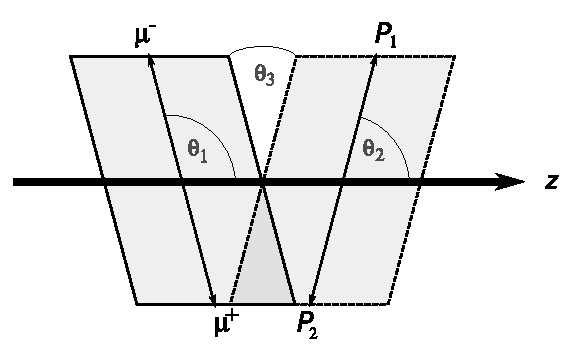
\includegraphics[width=.6\textwidth]{fig-topology.pdf}
    \caption{Decay topology for decays $B\to P_1 P_2 \ell_1 \bar\ell_2$. \label{fig:topology}\fred{We should use the same symbol $\theta$ as in text}}
\end{figure}

In several interesting processes we might only have an approximate
result for $P$.  In this section, we focus on one particular class of
mismodelling of the signal PDF: the angular momentum-cutoff in partial
wave expansions. This mismodelling potentially affects a large number
of decays and scattering processes. For the sake of clarity we take
the interesting class of four-body decays $B\to P_1 P_2 \ell_1
\bar\ell_2$ \fred{How general is this? The plot implies that the
  dimeson and the dilepton do not have a common vertex. But this
  requires an intermediate state, e.g., $K^{*}$}as an
example\footnote{This includes the rare $b\to s$ mediated $B$ decay $B
  \to K\pi\ell^+\ell^-$, and the $V_{ub}$ suppressed decay $B\to
  \pi\pi\ell^+\bar\nu_\ell$. For both examples the PDF $P$ is known in
  the small-width approximation and when assuming a pure $P$-wave,
  resonant final state. An extension to $S-P$ interference has been
  studied for $B\to K\pi\ell^+\ell^-$
  \cite{Blake:2012mb,Becirevic:2011bp}, and for $\bar{B}\to
  \pi\pi\ell^-\bar\nu_\ell$ \cite{Faller:2013dwa}. For a first study
  of $S$, $P$
  and $D$ interference, see \cite{Das:2014sra}}.\\

Within existing analyses, the PDFs of these decays are usually expressed in terms of one or a few
partial waves of the dimeson system. However, the angular momentum of the dimeson system is unbounded
from above, and gives rise to an infinite set of angular observables.\\

For the selected class of decays, we can describe that problem as follows: The PDF $P$ has a fixed dependence on the dilepton
helicity angle $\theta_1$ and the azimuthal angle $\theta_3$. (See also \refapp{btokpill} for details
on the angular distribution.) However, at the level of decay amplitudes the dimeson system can have an arbitrarily
large total angular momentum $j$; only its third component is restricted to $m = -1,0,+1$.
It is then usual to compute the angular distribution explicitly in terms of $\theta_1$ and $\theta_3$, but leave
the angular observables dependent on the remaining helicity angle $\theta_2$.
We advocate here that is a sensible procedure to perform an expansion in terms of Legendre polynomials $p_{j}^{(|m|)}$
with respect to the remaining angle $\theta_2$. Using the observables $S_k(\vec{\nu})$, $k=1,\dots,9$, with $\vec{\nu}=(q^2, k^2)$
and as defined in \refapp{partial-waves} \fred{A lot of mixing between appendices C and E}, the expansion reads
\begin{equation}
    S_{k}(\vec{\nu},\cos\theta_2) \equiv \sum_{j} \frac{1}{n_{j,|m|}} S_{k,j}(\vec{\nu}) p_{j}^{(|m|)}(\cos\theta_2)\sin\theta_2\,,
\end{equation}
where the the normalization factor $n_{j,|m|}$ is defined in \refeq{legendre-scalar-product}. Within our
example we have (cf. also \refapp{btokpill})
\begin{equation}
    |m| = \begin{cases}
        0\,, & k = 1,2,6\,\\
        1\,, & k = 3,4,5,7,8,9\,,
    \end{cases}\,.
\end{equation}
The angular observables $S_{k,j}$ defined as coefficients of this expansion in Legendre polynomials
have the merit of a well defined total angular momentum, and thus are physically discriminable.
As a consequence of the orthogonality of the Legendre polynomials, any mismodelling (or rather, lack of modelling of higher
partial-wave observables) \emph{does not affect} the method of moments as discussed in the previous section. To wit,
ignoring further (orthogonal) terms in the PDF cannot affect the mean vector $(\dots, S_k, \dots)$ nor its variance. \fred{yes!}\\

Unfortunately, this benefit on the experimental side is accompanied with a theoretical draw back. Each observable
$S_{k,j}(\vec{\nu})$ consists of an infinite sum of bilinears of partial-wave amplitudes. It remains for theoretical
analyses to estimate or calculate the impact of partial waves beyond the S and P wave contributions.
(For $B\to K\pi\ell^+\ell^-$ a first study has been carried out where contributions up to the D wave are studied \cite{Das:2014sra}).\\

We wish to emphasize, however, that detector acceptance effects systematically affect the expansion for any basis
of angular functions, including the one suggested in this section. The means to cope with this problem are discussed
in the following subsection.


\subsection{Recipe for the Determination of Detector Acceptance Effects}
\label{sec:systematics:acceptance}

The determination of a detector's performance to detect signal events
with accurate determination of the event's angles is generally a
difficult task. In the ideal case, one would have an explicit
probabilistic model of the detector acceptance effects and could thus
write down the full forward model from which the measured events
arise. In practice, this would require much more CPU time than
available, and one is therefore forced to simplify the model. The
standard approach is to generate the \emph{true} particle events
$\lbrace x_\text{t}^{(n)}\rbrace =
\lbrace(\vec{\nu}^{(n)}_\text{t},\vec\theta^{(n)}_\text{t})\rbrace$,
$n=1,\dots,N_\text{t}$, from a PDF assumed to describe the bare
physical process, and to propagate those particles through a detailed
simulation of the detector.  The observable traces that the particles
leave in the detector are fed into reconstruction algorithms resulting
in the \emph{detector} events $\lbrace x^{(n)}_\text{d}\rbrace =
\lbrace(\vec{\nu}^{(n)}_\text{d}, \vec\theta^{(n)}_\text{d})\rbrace$,
$n=1,\dots,N_\text{d}$.  In general, the distribution of the detected
events is
\begin{equation}
    P_\text{d}(x_\text{d}) = \int P_\text{t}(x_\text{t}) E(x_\text{d} | x_\text{t}) \rmdx{x_\text{t}}\,.
\end{equation}
Here $P_\text{t}$ is the probability distribution of the true events,
and the kernel $E(x_\text{d}| x_\text{t})$ parametrizes acceptance and
resolution effects. Note that $P_\text{d}$ is \emph{not} a PDF, since
it is not normalized,
\begin{equation}
    \int P_\text{d}(x) \rmdx{x} \neq 1\,.
\end{equation}
For the sake of clarity, we will restrict ourselves
to pure acceptance effects and suppress resolution effects in the remainder of this section; i.e.,
\begin{equation}
    E(x_\text{d}, x_\text{t}) \equiv \eps(x_\text{t}) \delta(x_\text{d}, x_\text{t})\,.
\end{equation}
We will refer to $\eps$ as the \emph{detector acceptance} function. In what follows,
we propose a systematic methods to unfold all effects of $\eps$ through MC simulations
and the method of moments.\\


We will now proceed with the explicit usage of a uniangular PDF with $x = \cos\theta$.\footnote{%
    The generalization of this section to multiangular PDFs is straighforward. It can be achieved
    by promoting $x$ to a vector, promoting the Legendre polynomials to products of independent polynomials
    or spherical harmonics, and promoting the indices $i,j,k,m$ to multi-indices.
}
Let us define the PDF in terms of the Legendre polymials (i.e., $f_k(x) \equiv P_k(x)$),
\begin{equation}
    P(x) \equiv \sum_k S_k f_k(x),
\end{equation}
where $k = 0, 1, \dots$ denotes the total angular momentum of the observables.
From the normalization of the PDF then follows $S_0 = 1/2$. From positivity of $P$ one
obtains $|S_k| \leq 1/2$ for angular momentum $k > 0$. More stringent relations between the
$S_k$ might hold, but are beyond the scope of this work. For latter use, we define
$\vec{S}^{(m)}_k \equiv 1/2 (\delta_{k,0} + \delta_{k,m})$, and we emphasize that
\begin{equation}
    P^{(m)}(x) \equiv P(x | \lbrace S^{(m)}_k \rbrace)
\end{equation}
is a PDF. The dual basis of angular functions follows then from the normalization
and orthogonality of the Legendre polynomials, and one therefore has
\begin{equation}
    \tilde{f}_k(x) = \frac{2 k + 1}{2} f_k(x),\qquad \int_{-1}^{+1} \tilde{f}_k(x) f_l(x) \rmdx{x} = \delta_{k,l}\,.
\end{equation}


We now define the \emph{simulated raw} moments $\lbrace Q_{i}^{(m)}\rbrace$,
\begin{equation}
    Q_i^{(m)} \equiv \int_{-1}^{+1} \tilde{f}_i(x) P^{(m)}(x) \eps(x) \rmdx{x} = \frac{1}{2} \int_{-1}^{+1} \tilde{f}_i(x) \big[f_0(x) + f_m(x)\big] \eps(x) \rmdx{x}\,,
\end{equation}
which are instrumental to our recipe. MC estimators for these simulated moments can be constructed from specifically crafted detector events $x_\text{d}^{(n,m)}$, $n = 1, \dots, N_\text{d}^{(m)}$, where
\begin{equation}
    x_\text{d}^{(n,m)} \sim P_\eps^{(m)} \equiv \frac{P^{(m)} \eps}{R^{(m)}}\,.
\end{equation}
Here the normalization $R^{(m)}$ is chosen such that $\int P_\eps^{(m)}(x) \rmdx{x} = 1$.
We emphasize that $R^{(m)}$ can estimated as $\est{R}^{(m)} = N_\text{d}^{(m)} / N_\text{t}$, where $N_\text{t}$ corresponds to the number of simulated true events.
The estimators then read
\begin{equation}
    \est{Q}_i^{(m)} \equiv \est{R}^{(m)} \frac{1}{N_\text{d}} \sum_n^{N_\text{d}} \tilde{f}_i(x_\text{d}^{(n,m)})
\end{equation}

Linearity of the integral over $x$ and convergence of the expansion of $P_\eps^{(m)}$ in terms Legendre polynomials ensures that
\begin{equation}
    Q_i^{(m)} = \sum_j M_{ij} S_j^{(m)}\,.
\end{equation}
We call the matrix $M_{ij}$ the \emph{unfolding matrix}, which is specific to our decay at hand. Given our definition of
$S_k^{(m)}$ it can easily be calculated as
\begin{equation}
    M_{ij} = \begin{cases}
        2 Q_i^{(0)}                          & j = 0\,,\\
        2\left(Q_i^{(j)} - Q_i^{(0)}\right)  & j \neq 0\,,\\
    \end{cases}
\end{equation}
and its MC estimator $\est{M}_{ij}$  can be obtained through the replacements $Q_i^{(m)} \to \est{Q}_i^{(m)}$.\\

In order to finally extract the angular observables from data, we use the \emph{measured raw moments}. Their MC estimator
$\lbrace \est{Q}_i\rbrace$ -- based on the \emph{detected events} $x^{(n)}$, $n=1,\dots,N$ -- reads
\begin{equation}
    \est{Q}_i \equiv R \frac{1}{N} \sum_n^N \tilde{f}_i(x^{(n)})\,.
\end{equation}
Here $R \equiv \int P(x) \eps(x)$ is an a priori unknown normalization that also occurs in the determination of the branching
ratio of the specific decay. We then obtain MC estimators of the angular observables via
\begin{equation}
    \est{S}_i \equiv \sum_{i} \left(\hat{M}^{-1}\right)_{ij} \est{Q}_j\,.
\end{equation}
The precise value of $R$ depends on the a priori unknown angular observables $\lbrace S_i\rbrace$.
However, ratios and other suitable combinations of the estimators $\lbrace \est{S}_i\rbrace$ are independent
of $R$.

It remains to be emphasized that the dimensionality of the raw angular observables is not completely
fixed by the number of angular momentum configurations of the process at hand. Let us revisit the
decay $B\to K\ell^+\ell^-$, with only one angle,  to clear this up. For $B\to K\ell^+\ell^-$, the
total angular momentum associated the dilepton pair can, at the level of observables, be either $0$,
$1$ or $2$. We assume now that the acceptance function $\eps$ can be conveniently expanded in terms
of Legendre polynomials up to maximal angular momentum $L$. From angular momentum conservation
follows immediately that $\dim Q = L + 2$, and thus the unfolding matrix $M$ will be of
dimension $L + 2 \times L + 2$. (For a multiangular distribution the maximum angular momentum
has to be determined in the same way for each angle.)
Since the $\eps$ depends highly on the nature of the particle detector at hand, it remains for
the experimental collaborations to determine the maximum order of such an expansion.

The accuracy of the unfolding process as outlined above critically depends on both the accuracy
of the detector simulation, as well as the uncertainties induced by the MC estimates. While
considerations of any detector simulation is beyond the scope of this work, we can, however,
comment on the MC-induced uncertainties. As usual, one needs to find a balance between
compute time and accuarcy. We find for a uniangular distribution and a total of $6\cdot 10^6$ MC
samples (i.e., $2 \cdot 10^6$ MC samples per row of $M_{ij}$) that the error on the mean is
smaller than $6\cdot 10^{-4}$. Let us conclude this section by commenting that the unfolding
matrix is universal in a sense. Specifically, it can be reused in analyses with a similar underlying decay.
Therefore, computing resources spent on improving its accuracy are therefore not wasted.


\section{Toy Studies}
\label{sec:numerics}

We now study the performance of the proposed method. In order to do so, we simulate
individual events for two separate physical processes: one uni-angular, and one tri-angular decay
distribution. We repeats theses analysis for varying sample sizes, ranging from
$50$ to $500$ events. Our toy analysis base on SM predictions for angular observables
in the decays $B\to K\ell^+\ell^-$ and $B\to K^*(\to K\pi)\ell^+\ell^-$, respectively.
In order to faithfully investigate the performance of the method of moments, we repeats our
numerical studies for several bin sizes in the kinematic range $1 \GeV^2 \leq q^2 \leq 6\GeV^2$,
as well as $15 \GeV^2 \leq q^2 \leq q^2_\text{max}$. Here, the bin size is chosen either
as $1\GeV^2$ or $0.5\GeV^2$. This setup is meant to ensure that a wide spectrum of possible
values for the angular observables is investigated.\\

Our finding can be summarized as follows:
\begin{itemize}
    \item In all studied cases we observed not a single bias in the distribution of the $\mathrm{pull}$
        of any observables $S$,
        \begin{equation}
            \mathrm{pull_i} \equiv \frac{\est{S} - S}{\est{\sigma}_S}\,.
        \end{equation}
        Here $S$ refers to the true (input) value for the angular observables, $\est{S}$ refers to the
        MC estimate, and $\est{\sigma} \equiv \sqrt{\est{\Sigma}}$ refers to an estimator of the
        variance of the measurement. All pull distributions obtained in our studies can be successfully
        fitted to a gaussian distribution. Due to the large number of studied distributions, we have
        to restrict ourselved to a subset. In our opinion the pull distributions for the observables
        $S_5 \simeq 27\%$ and $S_7 \simeq 2\%$, which are obtained from SM-like $B\to K^*\ell^+\ell^-$
        decays, are good examples. We show their respective pull distributions for \danny{$XXX$} toy studies
        of $200$ events per study in \reffig{pulls}.
    \item We study the absolute uncertainty $\sigma_k(K)$ with respect to the angular observable $S_k$
        as a function of the number of simulated events $K$. As expected for a multivariate gaussian
        distribution, we find that the absolute uncertainty is well fitted by
        \begin{equation}
            \label{eq:unc-on-mean}
            \sigma_k(K) = \frac{\sigma_k(1)}{\sqrt{K}}
        \end{equation}
        with $\sigma_k(1) = \order{1}$, regardless of the absolute size of $S_k$. The latter can best be shown
        for the example of uncertainties of two observables. Taking again $S_5$ ($\simeq 27\%$) and $S_7$ ($\simeq 2\%$)
        for SM-like $B\to K^*\ell^+\ell^-$ decays, we show the absolute uncertainty in \reffig{errors}.
    \item For all toy studies, we produce plots of their skewness and their kurtosis as functions of
        $N$. We find in all cases that the mean skewness and kurtosis converge towards zero.
        \todo{Plot Skewness and Kurtosis for $S_5$ and $S_7$ as functions of the number of simulated events $K$.}
\end{itemize}
All results of our toy studies, as summarised above, show consistently that the joint distribution of the angular
observables converges towards a multivariate Gaussian distribution. We therefore propose to describe the
resulting distribution as a multivariate Gauss when skewness and kurtosis fall below a given threshold.
The precise target threshold for skewness and kurtosis are subject to the details of the underlying physical analysis, and reside therefore outside the scope of this work.

\begin{figure}[t]
        \centering
            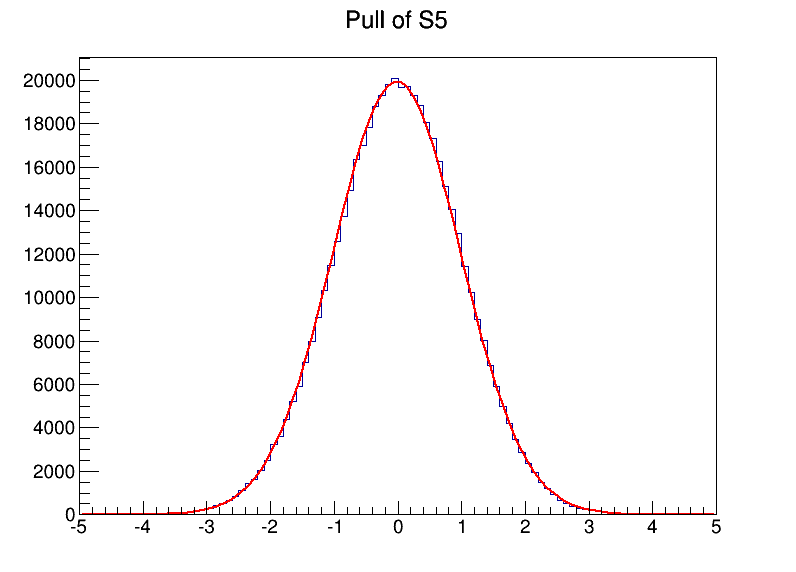
\includegraphics[width=0.45\textwidth]{figs/pull-Q2_5_6_S5_200.png}
            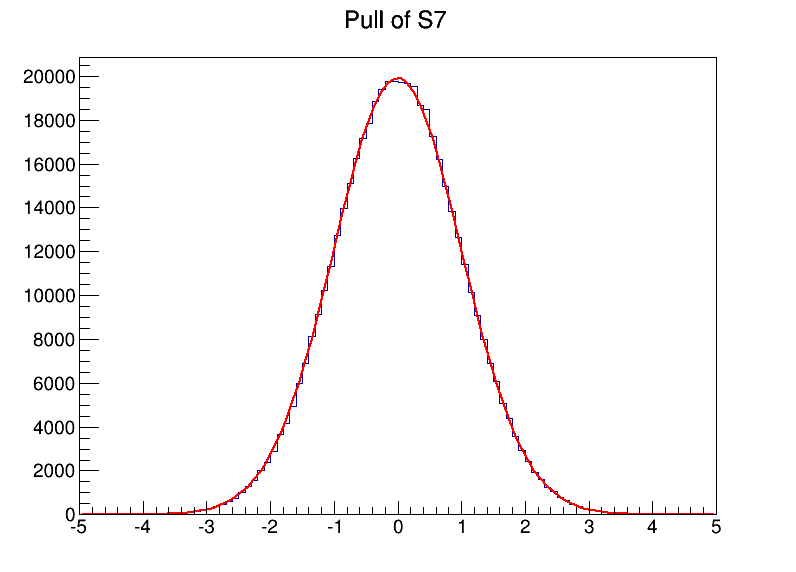
\includegraphics[width=0.45\textwidth]{figs/pull-Q2_5_6_S7_200.png}
        \caption{Pull distribution for the angular observables $S_5$ and $S_7$, extracted from $200$ simulated events of the decay $B\to K^*\ell^+\ell^-$. The red curve represents a fit to a gaussian distribution.}
        \label{fig:pulls}
\end{figure}

\begin{figure}[t]
        \centering
            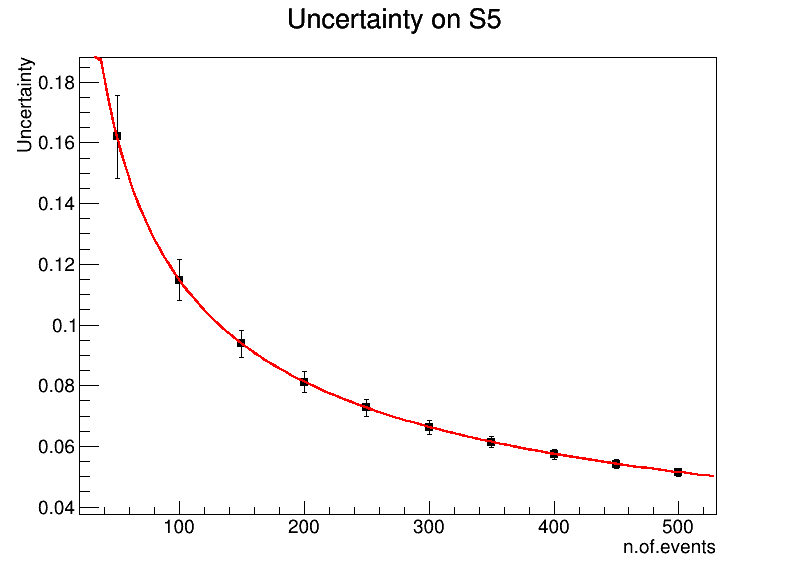
\includegraphics[width=0.45\textwidth]{figs/error-Q2_5_6_S5.png}
            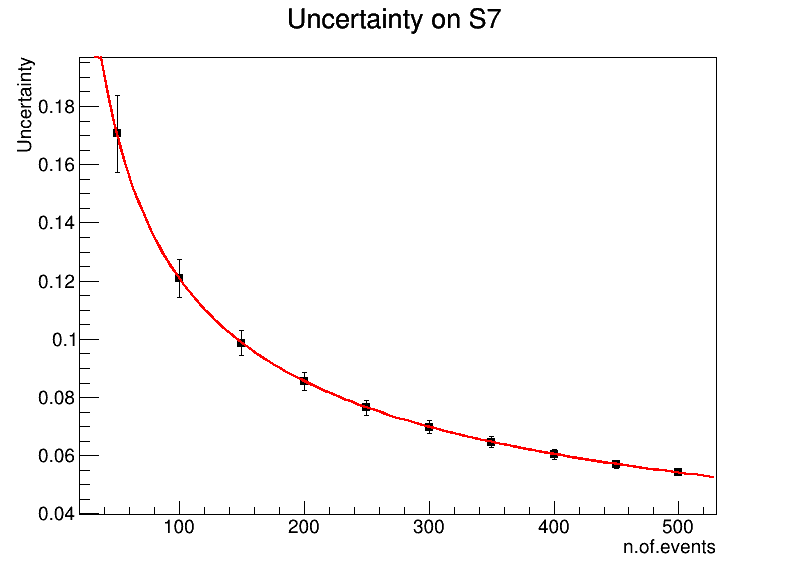
\includegraphics[width=0.45\textwidth]{figs/error-Q2_5_6_S7.png}
            \caption{Uncertainty of the angular observables $S_5$ and $S_7$, extracted from simulated events of the decay $B\to K^*\ell^+\ell^-$ and as a function of the number of simulated events $K$. The red curve represents a fit to the function given in \refeq{unc-on-mean}.}
        \label{fig:errors}
\end{figure}

\section{Conclusion}

We have carried out a combined analytical and numerical study of the method of moments; a method for
the extraction of angular observales from the angular distribution of a generic multi-body process.
We have studied the performance of the method of moments using pseudo data derived from the SM
predctions for one uniangular decay ($B\to K\ell^+\ell^-$) and one triangular decay ($B\to K^*\ell^+\ell^-$).
From this, we find rapid convergence of the joint likelihood of the angular observables towards a multivariate Gaussian.
We draw the conclusion that this method exhibits several benefits in the determination of angular observables when
compared with a maximum-likelihood fit.\\

First, we find no bias in the determinations of the angular observables even for a small number of events.
However, this comes at the expense of a slight increase of the order of $10\%$\todo{check!} for the statistical uncertainty
on the mean.
Second, in the absence of acceptance effects, a determination using the method of moments is correct and unbiased
even when not all aspects of the physical distribution are modelled. This is explicitl shown for the case of
higher partial waveds in multibody final states.
Third, we develop a systematic method for the dertermination of detector acceptance effects that lead to
dilution and mixing of the angular observables. We present a way to calculate the necessary unfolding matrix,
which is only computationally feasible when using the method of moments.\\
Fourth, the fact that the joint distribution of the results is Gaussian allows for an easy transfer of correlation
information to theory analyses.
Last but not least, the resulting distribution arises without additional constraints necessary for the convergence
of some maximum-likelihood fits. Therefore the results can be directly combined with similarly-obtained results from
a different experiment, without the need to remove the constraints of measurements that stem from different experiments.\\

In conclusion, we argue that the method of moments is a competetive alternative to maximum-likelihood fits as long
as angular distributions are involved. We wish to raise the interesting prospect of extending this very method to
applications with non-angular orthogonal bases for the PDF.


\acknowledgments

The work of D.v.D has been supported by the Bundesministerium f\"ur Bildung und Forschung (BMBF).
We would like to thank Ulrik Egede and Konstantinos Petridis for insightful discussions.
\danny{Potential people to read the manuscript: Jochen Dingfelder (Belle-II, Bonn), Ulrik Egede (LHCb, Imperial London), Christoph Langenbruch (LHCb, Warwick), Michel De Cian (LHCb, Heidelberg), Adrian Bevan (ATLAS, Queen Mary)  }
D.v.D would like to thank Gudrun Hiller and Martin Jung for discussing the results of \cite{Das:2014sra} prior to publication.

\appendix

\section{Application to $\bar{B}\to\bar{K}\ell^+\ell^-$}
\label{app:btokll}

The PDF for the decay $\bar{B}\to\bar{K}\ell^+\ell^-$ has been calculated for the most
complete basis of dimension-six $b\to s \ell^+\ell^-$ operators. It reads \cite{Bobeth:2007dw,Bobeth:2012vn}
\begin{equation}
    P(q^2, \cos\theta_1)
        = \frac{1}{\rmdx{\Gamma}/\rmdx{q^2}} \frac{\rmdx{^2\Gamma}}{\rmdx{q^2} \rmdx{\cos\theta_1}}
        = \frac{a(q^2)}{\rmdx{\Gamma}/\rmdx{q^2}} + \frac{b(q^2)}{\rmdx{\Gamma}/\rmdx{q^2}} \cos\theta_1 + \frac{c(q^2)}{\rmdx{\Gamma}/\rmdx{q^2}} \cos^2\theta_1
        = \sum_i S_i p_i(\cos\theta_1)\,,
\end{equation}
with the conventional observables $a(q^2)$ through $c(q^2)$, and $\rmdx{\Gamma}/\rmdx{q^2} = 2a + 2/3 c$. We conveniently use the Legendre polynomials
$p_i(x)$, $i=0,1,2$,
\begin{equation}
\begin{aligned}
    p_0(x) & = 1\,, &
    p_1(x) & = x\,, &
    p_2(x) & = \frac{1}{2} (3x^2 - 1)\,,
\end{aligned}
\end{equation}
as our basis of angular functions. Our basis of angular observables then
translates to the conventional basis as
\begin{equation}
\begin{aligned}
    S_0 & = \frac{1}{2}\,, &
    S_1 & = \frac{b}{\Gamma}\,, &
    S_2 & = \frac{2c}{3\Gamma}\,.
\end{aligned}
\end{equation}
In this case, the dual basis is simply given by $\tilde{p}_i(x) = (2 i + 1)/2 p_i(x)$
such that
\begin{equation}
    \int_0^\pi \rmdx{\theta_1} \dual{p}_i(\cos\theta_1) P(q^2, \cos\theta_1)\sin\theta_1 = S_i(q^2)\,.
\end{equation}

\section{Application to $\Lambda_b\to \Lambda(\to N \pi)\ell^+\ell^-$}
\label{app:lambdabtolambdall}

The PDF for the decay --- in the presence of Standard-Model operators and their chirality-flipped counter parts --- reads \cite{Boeer:2014xx}
\begin{equation}
    P(q^2, \cos\theta_1, \cos\theta_2, \theta_3) = \frac{1}{\rmdx{\Gamma} /\, \rmdx{q^2}} \frac{\rmdx{^4\Gamma}}{\rmdx{q^2} \rmdx{\cos\theta_1} \rmdx{\cos\theta_2} \rmdx{\theta_3}} = \sum_i S_i f_i(\cos\theta_1, \cos\theta_2, \theta_3)\,,
\end{equation}
where $q^2$ denotes the dilepton mass squared, $\theta_1 \equiv \theta_\ell$ and $\theta_2 \equiv \theta_\Lambda$ denote the
helicity angles in the dilepton and
$N\pi$ systems, respectively, and $\theta_3 = \phi$ denotes the azimuthal angle.
The index $i$ should be interpreted as a multi-index, $i \equiv (l_1, l_2, m)$,
where $0 \leq l_1 \leq 2$ and $0 \leq l_2 \leq 1$ denote the total angular momentum in the
dilepton and the $N\pi$ system, respectively, and $-1 \leq m \leq 1$
is the third component of either of the angular momenta.
Our choice of an orthonormal basis and its dual reads
\begin{equation}
\label{eq:lambdab:bases}
\begin{aligned}
    f_{l_1, l_2, m}(\cos\theta_1, \cos\theta_2, \theta_3)
    & = \sqrt{\frac{(l_1 - |m|)!\,(l_2 - |m|)!}{(l_1 + |m|)!\,(l_2 + |m|)!}} p_{l_1}^{|m|}(\cos\theta_1) p_{l_2}^{|m|}(\cos\theta_2)\\
    & \times \begin{cases}
            \cos(|m|\theta_3) & m > 0\\
            \sin(|m|\theta_3) & m < 0\\
            1                 & m = 0
        \end{cases}\,,\\
    \tilde{f}_{l_1, l_2, m}(\cos\theta_1, \cos\theta_2, \theta_3)
    & = \frac{(2l_1 + 1)(2l_2 + 1)}{8\pi}\sqrt{\frac{(l_1 - m)!\,(l_2 - m)!}{(l_1 + m)!\,(l_2 + m)!}} p_{l_1}^m(\cos\theta_1) p_{l_2}^m(\cos\theta_2)\\
    & \times \begin{cases}
            2 \cos(|m|\theta_3) & m > 0\\
            2 \sin(|m|\theta_3) & m < 0\\
            1                   & m = 0
        \end{cases}\,.\\
\end{aligned}
\end{equation}
The correspondence between out choice of angular observables in the angular momentum basis, and the angular
observables as defined in reference \cite{Boeer:2014xx} reads
\begin{equation}
\begin{aligned}
    8\pi S_{0, 0,  0} & = 1\,,                                                             &
    8\pi S_{1, 0,  0} & = \frac{3 K_{1c}}{\rmdx\Gamma/\rmdx{q^2}}\,,                       &
    8\pi S_{2, 0,  0} & = \frac{2(K_{1cc} - K_{1ss})}{\rmdx\Gamma/\rmdx{q^2}}\,,           \\
    8\pi S_{0, 1,  0} & = \frac{K_{2cc} + 2 K_{2ss}}{\rmdx\Gamma/\rmdx{q^2}}\,,            &
    8\pi S_{1, 1,  0} & = \frac{3 K_{2c}}{\rmdx\Gamma/\rmdx{q^2}}\,,                       &
    8\pi S_{2, 1,  0} & = \frac{2(K_{2cc} - K_{2ss})}{\rmdx\Gamma/\rmdx{q^2}}\,,           \\
                 &                                                                    &
    8\pi S_{1, 1, -1} & = \frac{6 K_{4s}}{\rmdx\Gamma/\rmdx{q^2}}\,,                       &
    8\pi S_{2, 1, -1} & = \frac{2 \sqrt{3} K_{4sc}}{\rmdx\Gamma/\rmdx{q^2}}\,,             \\
                 &                                                                    &
    8\pi S_{1, 1, +1} & = \frac{6 K_{3s}}{\rmdx\Gamma/\rmdx{q^2}}\,,                       &
    8\pi S_{2, 1, +1} & = \frac{2 \sqrt{3} K_{3sc}}{\rmdx\Gamma/\rmdx{q^2}}\,,
\end{aligned}
\end{equation}
where the decay width is
\begin{equation}
    \frac{\rmdx{\Gamma}} {\rmdx{q^2}} = 2 K_{1ss} + K_{1cc}\,.
\end{equation}

The dual basis is chosen such that
\begin{equation}
    \int_{-1}^{+1} \rmdx{\cos \theta_1} \int_{-1}^{+1} \rmdx{\cos \theta_2} \int_0^{2\pi} \rmdx{\theta_3} P(q^2, \cos \theta_1, \cos \theta_2, \theta_3) \dual{f}_i(\cos \theta_1, \cos \theta_2, \theta_3) = S_i(q^2)\,.
\end{equation}

For the purpose of unfolding acceptance effects as laid down in \refsec{systematics:acceptance}, it is instrumental
to know that $f_{0,0,0} \equiv 1$, and that $\max_{\cos\theta_1,\cos\theta_2,\phi} |f_{l_1, l_2, m}| < 1$.
The recipe's generating PDFs are therefore
\begin{equation}
    P(x|\lbrace S_i^{(j)}\rbrace)\,,\quad\text{with}\quad S_i^{(j)} = \frac{1}{8\pi}\left(\delta_{i,(0,0,0)} + \delta_{i,j}\right)\,,
\end{equation}
where $j$ ís now also a multi-index representing $j \equiv (\tilde l_1, \tilde l_2, \tilde m)$.

\section{Application to $\bar{B}\to\bar{K}\pi\ell^+\ell^-$}
\label{app:btokstarll}

The PDF for the decay $\bar{B}\to\bar{K}\pi\ell^+\ell^-$ --- up to and including P-wave contributions --- has been calculated
for the most general basis of dimension-six $b\to s$ operators. It reads, expressed in terms of the angular observables $\lbrace J_i\rbrace$ \cite{Blake:2012mb,Bobeth:2012vn}
\begin{equation}
    P(q^2, \cos\theta_1, \cos\theta_2, \theta_3) = \frac{1}{\rmdx{\Gamma}/\rmdx{q^2}} \frac{\rmdx{^4\Gamma}}{\rmdx{q^2} \rmdx{\cos\theta_1} \rmdx{\cos\theta_2} \rmdx{\theta_3}}
    = \sum_i S_i(q^2) f_i(\cos\theta_1, \cos\theta_2, \theta_3)\,,
\end{equation}
where $\theta_1 \equiv \theta_\ell$ is the dilepton helicity angle; $\theta_2 \equiv \theta_{K}$ is the $\bar{K}\pi$ helicity angle; $\theta_3 \equiv \phi$ is the azimuthal angle;
and $q^2$ is the square of the dilepton mass. The $q^2$-differential decay width reads
\begin{equation}
    \frac{\rmdx{\Gamma}}{\rmdx{q^2}} = \frac{\big(3 J_{1c} - J_{2c}\big) + 2\big(3J_{1s} - J_{2s}\big)}{3}\,.
\end{equation}
It is convenient to define the basis of angular functions and its dual in terms of
associated Legendre polynomials $p_l^m(x)$. The index $i$ should thus be interpreted as a multi-index
, $i \equiv (l_1, l_2, m)$, where $0 \leq l_1 \leq 2$ and $0 \leq l_2 \leq 2$ denote the total angular
momentum in the dilepton and the $K\pi$ system, respectively, and $-2 \leq m \leq 2$
is the third component of either of the angular momenta.
We use the same bases of angular functions as given in \refeq{lambdab:bases} for the decay $\Lambda_b\to \Lambda\ell^+\ell^-$.
In that case, the angular observables correspond to the usual choice of observables via
\begin{equation}
\begin{aligned}
    8\pi S_{0, 0,  0} & = 1\,,                                                                             &
    8\pi S_{0, 1,  0} & = \frac{3 J_{1i} - J_{2i}}{\rmdx{\Gamma}/\rmdx{q^2}}\,,                            &
    8\pi S_{0, 2,  0} & = \frac{6 (J_{1c} - J_{1s}) - 2(J_{2c} - J_{2s})}{3\rmdx{\Gamma}/\rmdx{q^2}}\,,
\end{aligned}
\end{equation}
and
\begin{equation}
\begin{aligned}
%
                      &                                                                                    &
    8\pi S_{1, 1, -1} & = \frac{6 J_{7i}}{\rmdx{\Gamma}/\rmdx{q^2}}\,,                                     &
    8\pi S_{1, 2, -1} & = \frac{4 \sqrt{3} J_{7}}{\rmdx{\Gamma}/\rmdx{q^2}}\,,                             \\
%
    8\pi S_{1, 0,  0} & = \frac{J_{6c} + 2 J_{6s}}{\rmdx{\Gamma}/\rmdx{q^2}}\,,                            &
    8\pi S_{1, 1,  0} & = 0\,,                                                                             &
    8\pi S_{1, 2,  0} & = \frac{2(J_{6c} - J_{6s})}{\rmdx{\Gamma}/\rmdx{q^2}}\,,                           \\
%
                      &                                                                                    &
    8\pi S_{1, 1, +1} & = \frac{6 J_{5i}}{\rmdx{\Gamma}/\rmdx{q^2}}\,,                                     &
    8\pi S_{1, 2, +1} & = \frac{4 \sqrt{3} J_{5i}}{\rmdx{\Gamma}/\rmdx{q^2}}\,,
\end{aligned}
\end{equation}
and
\begin{equation}
\begin{aligned}
%
                 &                                                                                    &
                 &                                                                                    &
    8\pi S_{2, 2, -2} & = \frac{8 J_9}{\rmdx{\Gamma}/\rmdx{q^2}}                                           \\
%
                 &                                                                                    &
    8\pi S_{1, 2, -1} & = \frac{6 J_{?}}{\rmdx{\Gamma}/\rmdx{q^2}}\,,                                      &
    8\pi S_{1, 2, -1} & = \frac{4 \sqrt{3} J_{?}}{\rmdx{\Gamma}/\rmdx{q^2}}\,,                             \\
%
    8\pi S_{2, 0,  0} & = \frac{4 (J_{2c} + 2 J_{2s})}{\rmdx{\Gamma}/\rmdx{q^2}}\,,                        &
    8\pi S_{2, 1,  0} & = \frac{4 J_{2i}}{\rmdx{\Gamma}/\rmdx{q^2}}\,,                                     &
    8\pi S_{2, 2,  0} & = \frac{8 (J_{2c} - J_{2s})}{3 \rmdx{\Gamma}/\rmdx{q^2}}\,,                        \\
\end{aligned}
\end{equation}

As before, for the purpose of unfolding acceptance effects as laid down in \refsec{systematics:acceptance}, it is instrumental
to know that $f_{0,0,0} \equiv 1$, and that $\max_{\cos\theta_1,\cos\theta_2,\phi} |f_{l_1, l_2, m}| \leq 1$.
The recipe's generating PDFs are therefore
\begin{equation}
    P(x|\lbrace S_k^{(j)}\rbrace)\,,\quad\text{with}\quad S_k^{(j)} = \frac{1}{8\pi}\left(\delta_{k,0} + \delta_{k,j}\right)\,,
\end{equation}
where also $j$ is now a multi-index representing $j \sim (l_1, l_2, m)$.


\section{On the Partial-Wave Expansions of Angular Observables}
\label{app:partial-waves}

Let us assume that the angular decomposition has been achieved for some
PDF $P$ for all angles except one, which we label $\theta$. We now focus on only of of the resulting
observables, which we label $S(\theta) \equiv S(\vec{\nu},\theta)$. The dependence on the non-angular
variables will be suppressed in the following. \danny{Fred: is this less confusing now?}
Further, let $S$ have an expansion in terms of partial waves
$l_1, l_2 = 0,1,2,\dots \hat{=}$ S,P,D$,\dots$ of the underlying amplitudes $A_1$ and $A_2$,
\begin{equation}
    \label{eq:def-partial-wave-observable}
    S(\theta) \equiv F\left[A_1(\theta) A_2^*(\theta)\right] \equiv F\left[\left(\sum_{l_1=0}^\infty A_1^{(l_1)} p_{l_1}^{(m_1)}(\cos\theta)\right) \left(\sum_{l_2=0}^\infty A_2^{*(l_2)} p_{l_2}^{(m_2)}(\cos\theta)\right)\right]\,,
\end{equation}
where $F \in \{\text{Re},\text{Im}\}$ denotes taking either the real
or the imaginary part. Here $p_{l}^{(m)}$ denotes an \emph{associated Legendre} polynomial and $m_i$ is the third component of the angular momentum of the amplitude $A_i$, and we impose $m_1 \geq m_2$.\\

From the positivity of amplitudes, one immediately finds
\begin{equation}
    \int \rmdx{\cos\theta}  \, |A_i(\theta)|^2 = \sum_{l_i = 0}^\infty |A_i^{(l_i)}|^2 n_{l_i, m_i} < \infty\,,
\end{equation}
where we introduce $n_{l,m}$ via the scalar product of two associated Legendre polynomials,
\begin{equation}
    \label{eq:legendre-scalar-product}
    n_{l, m} \delta_{l, l'} \equiv \int_{-1}^1 \rmdx{\cos\theta} p_{l}^{(m)}(\cos\theta) p_{l'}^{(m)} (\cos\theta)  = \frac{2}{(2 l + 1)} \frac{(l + m)!}{(l - m)!} \delta_{l, l'}\,.
\end{equation}
Using the large-$l$ behaviour of $n_{l,m}$ one finds that with increasing $l_i$ the partial-wave amplitudes must asymptotically fall off as \fred{Let's say why. Unitarity?} \danny{Finiteness of observables, so yes: unitarity!}
\begin{equation}
    |A_i^{(l_i)}(\cos\theta)| \Big|_{l_i \gg m_i} \sim \frac{1}{\sqrt{l_i}}\,.
\end{equation}
This motivates to cut off the partial-wave expansion at some arbitrary angular momentum $L$.\\

Will will show in the following that such a cut off
is compatible with defining a basis of angular observables as coefficients of Legendre polynomials in $\cos\theta$. Since this expansion implies
a well defined total angular momentum for each observable, one ensures that the observables can in fact be disentangled experimentally.\\

We propose the decomposition of $S$ in terms of the associated Legendre polynomials $p_{j}^{(m)}(\cos\theta)$, with total angular momentum $j$ and its third component $m=m_1 + m_2$.
\begin{equation}
    S(\theta) = \sum_j S_{j,m} p_{j}^{(m)}(\cos\theta)\,.
\end{equation}
This parametrization has two merits. First, we can immediately project out the angular observables $S_{j,m}$ by means of \refeq{legendre-scalar-product}:
\begin{equation}
    S_{j,m} = \frac{1}{n_{j,m}} \int_{-1}^{+1} \rmdx{\cos\theta} S(\theta) p_{j}^{(m)}(\cos\theta)\,.
\end{equation}
(Here and in the next step we may exchange the integral and the
series because each element of the series is a product of
polynomials on the compact support [-1,1], and thus each integral
is absolutely convergent).
Second, we can immediately express $S_{j,m}$ in terms of
the partial-wave amplitudes,
\begin{equation}
    \label{eq:partial-wave-observable-infinite}
    \begin{aligned}
        S_{j,m}
            & = \frac{1}{n_{j,m}} \int_{-1}^{+1} \rmdx{\cos\theta} p_{j}^{(m_1 + m_2)}(\cos\theta) \sum_{l_1,l_2=0}^\infty F\left[A_{1}^{l_1} p_{l_1}^{(m_1)}(\cos\theta) A_{2}^{*(l_2)}p_{l_2}^{(m_2)}(\cos\theta)\right]\\
            & = \sum_{l_1,l_2=0}^\infty F\left[A_{1}^{l_1} A_{2}^{*(l_2)}\right] \frac{T_{l_1,l_2,j}^{(m_1,m_2)}}{n_{j,m}}\,,\qquad\text{with }m = m_1 + m_2\,.
    \end{aligned}
\end{equation}

In the last step, we use Gaunt's formula \cite{Gaunt:1929} to integrate a triple product of associated Legendre polynomials,
\begin{equation}
\begin{aligned}
    T_{l_1,l_2,j}^{(m_1,m_2)}
        & = \int_{-1}^{+1} \rmdx{\cos\theta} p_{j}^{(m_1 + m_2)}(\cos\theta) p_{l_1}^{(m_1)}(\cos\theta) p_{l_2}^{(m_2)}(\cos\theta)\\
        & = (-1)^{s - l_1 - m_2} \frac{2 (l_1 + m_1)! (l_2 + m_2)! (2s - 2 l_2)! s!}{(l_1 - m_1)! (s - j)! (s - l_1)! (s - l_2)! (2s + 1)!}\\
        & \times \sum_{t=p}^q (-1)^t \frac{(j + m + t)!(l_1 + l_2 - m - t)!}{t! (j - m - t)! (l_1 - l_2 + m + t)! (l_2 - m_2 - t)!}\,,
\end{aligned}
\end{equation}
where
\begin{equation}
\begin{aligned}
    m & = m_1 + m_2\,, &
    m_1 & \geq m_2\,,  \\
    j, l_1, l_2 & \geq 0\,, &
    m, m_1, m_2 & \geq 0\,,
\end{aligned}
\end{equation}
and
\begin{equation}
\begin{aligned}
    s & = \frac{j + l_1 + l_2}{2}\,, &
    p & = \max(0, l_2 - l_1 - m)\,, &
    q & = \min(l_1 + l_2 - m, j - m, l_2 - m_2)\,.
\end{aligned}
\end{equation}
The necessary conditions for $T \neq 0$ are
\begin{equation}
    \label{eq:angular-momentum-addition}
    s \in \mathbb{N}\qquad \wedge \qquad l_1 - l_2 \leq l \leq l_1 + l_2,.
\end{equation}
The latter condition is well known from the addition rules of angular momenta. Note, however, that
the sum in \refeq{def-partial-wave-observable} goes to infinitely high angular momenta $l_1$ and $l_2$. As a consequence
of this and of \refeq{angular-momentum-addition}, the angular observables $P_{j,m}$
consist of sums with infinitely many terms. It is then up to theoretical analyses to
estimate or calculate the impact of individual contributions, with or without the cut off $L$.
For such an analysis in the decay $B\to K\pi\ell^+\ell^-$ we refer to \cite{Das:2014sra}.
We close by remarking that for any angular-momentum cut off $l < L$\fred{Do you mean $L < \infty$?}, one can find an upper limit for the squared sum of all remaining partial waves through a comparison with the inclusive decay
width.


\bibliography{references}

\end{document}
